\documentclass{classrep}
\usepackage[utf8]{inputenc}
\usepackage{color}
\usepackage{graphicx}
\usepackage{url}
\usepackage{hyperref}

\studycycle{Informatyka, studia STACJONARNE, I st.}
\coursesemester{VI}

\coursename{Komputerowe systemy rozpoznawania}
\courseyear{2020/2021}

\courseteacher{prof. dr hab. inż. Adam Niewiadomski}
\coursegroup{poniedziałek, 12:00}

\author{
  \studentinfo{Julia Szymańska}{224441} \and
  \studentinfo{Przemysław Zdrzalik}{224466} }

\title{Projekt 2.  Podsumowania lingwistyczne relacyjnych baz danych}

\begin{document}
\maketitle

%%%%%%%%%%%%%%%%%%%%%%%%%%%%%%%%%%%%%%%%
\section{Cel}
Celem projektu jest stworzenie aplikacji pozwalającej na generowanie podsumowań lingwistycznych w oparciu o kwantyfikatory rozmyte, co oznacza opisanie danych liczbowych ze zbioru danych\cite{dane} językiem quasi-naturalnym - pozornie naturalnym. Przykładem podsumowania lingwistycznego może być: X przedmiotów jest Y [P] - "Wiele wypadków jest przy ujemnej temperaturze [0,76]" oraz X przedmiotów będących Z jest Y [P] - "Wiele wypadków będących podczas deszczu, jest przy ujemnej temperaturze [0.68]".  Analizowany zbior danych zawiera liczbowe informacje o ponad 3 milionach wypadków samochodowych w 49 stanach Zjednoczonych Stanów Ameryki, mających miejsce od lutego 2016 do grudnia 2020\cite{dane}. Zbiór danych składa się z 47 kolumn. W tym celu wykonania podsumowania lingwistycznego zostaną wykorzystane metody logiki rozmytej\cite{fuzzy}. Logika rozmyta pozwala na opisanie wartości zapisanych językiem naturalnym za pomocą zrozumiałych określeń jak: mało, dużo, około połowy. W projekcie zostaną wykorzystane kwantyfikatory lingwistyczne względne takie jak: niewiele, około połowy oraz kwantyfikatory lingwistyczne absolutne takie jak: około jednego, około stu.


%%%%%%%%%%%%%%%%%%%%%%%%%%%%%%%%%%%%%%%%
\section{Charakterystyka podsumowywanej bazy danych}
W programie został użyty zbiór danych\cite{dane} znajdujący się w pliku CSV, który został przekształcony w bazę danych. 

Zbiór danych zawiera informacje o ponad 3 milionach wypadków samochodowych w 49 stanach Zjednoczonych Stanów Ameryki, mających miejsce od lutego 2016 do grudnia 2020. Spośród 47 kolumn znajdujących się w zbiorze danych, wybraliśmy następujące 11 kolumn:
\begin{itemize}
\item Czas rozpoczęcia - Start\_Time - czas rozpoczęcia się wypadku w lokalnej strefie czasowej, przyjmuje wartości od 8 lutego 2016, do 31 grudnia 2020. Wartość kolumny zostanie zamieniona na wartość całkowitą oznaczającą liczbę sekund od początku 1970 roku.
\item Czas zakończenia - End\_Time - czas zakończenia się wypadku w lokalnej strefie czasowej, przyjmuje wartości od 8 lutego 2016, do 1 stycznia 2021. Wartość kolumny zostanie zamieniona na wartość całkowitą oznaczającą liczbę sekund od początku 1970 roku. 
\item Odległość - Distance - długość odcinka ulicy wyrażony w milach, na którego miał wpływ wypadek. Przyjmuje wartości zmiennoprzecinkowe od 0 do 334, gdzie zdecydowana większość danych mieści się w przedziale od 0.00 do 4.00. 
\item Temperatura - Temperature - temperatura powietrza wyrażona w Fahrenheit'ach, w momencie, gdy zdarzył się wypadek.  Przyjmuje wartości zmiennoprzecinkowe od -16.00 do 104.00.  Temperature można opisac jako bardzo zimną, zimną, umiarkowaną, ciepłą, bardzo ciepłą. Oczywiście jest to opis subiektywny.
\item Temperatura odczuwalna - Wind\_Chill - temperatura odczuwalna wyrażona w Fahrenheit'ach, w momencie, gdy zdarzył się wypadek.  Przyjmuje wartości zmiennoprzecinkowe od -16.00 do 101.00. Temperaturę odczuwalną mozna opisać tak samo jak temperaturę.
\item Wilgotność - Humidity - wilgotność powietrza wyrażona w procentach w momencie, gdy zdarzył się wypadek. Przyjmuje wartości zmiennoprzecinkowe od 4.00 do 100.00. 
\item Ciśnienie - Pressure - ciśnienie powietrza wyrażone w inches, w momencie, gdy zdarzył się wypadek. Przyjmuje wartości zmiennoprzecinkowe od 27.00 do 32.00. Ciśnieje można opisac jako wysokie, umiarkowane lub niskie. 
\item Widoczność - Visibiity - widoczność wyrażona w milach, w momencie, gdy zdarzył się wypadek. Przyjmuje wartości zmiennoprzecinkowe od 0.00 do 12.00. 
Widoczność mozna opisać jako dobrą, ograniczoną, słabą.
\item Prędkość wiatru - Wind\_Speed - prędkość wiatru wyrażona w milach na godzinę,  w momencie, gdy zdarzył się wypadek. Przyjmuje wartości zmiennoprzecinkowe od 0.00 do 40.00. Wiatr mozna opisać jako słaby, umiarkowany, silny.
\item Ilość opadów - Principation - ilość opadów wyrażona w inches, w momencie, gdy zdarzył się wypadek. Jeśli opady nie występowały to kolumna przyjmuje wartość nan.  Przyjmuje wartości zmiennoprzecinkowe od 0.00 do 0.50.
\end{itemize}
\ \\
Atrybutom nadawane są opisane zwyczajowe wartości lingwistyczne ze względu na zwiększenie przystępności i ułatwienie szybkiego zrozumienia atrybutu przez człowieka, kiedy ten atrybut nie musi być dokładnie opisany.
Przykładowo temperatura, mimo że zrozumiała dla człowieka w postaci liczbowej, jest łatwiejsza do szybszego zrozumienia w postaci tekstowej, a dla ludzi nie ma dużego znaczenia czy temperatura rózni się o 1 czy 2 stopnie, wystarczy opisać ją słownie tak jak wcześniej podaliśmy jako  bardzo zimną, zimną, umiarkowaną, ciepłą, bardzo ciepłą.

\newpage
\begin{figure}[h!]
 \centering
 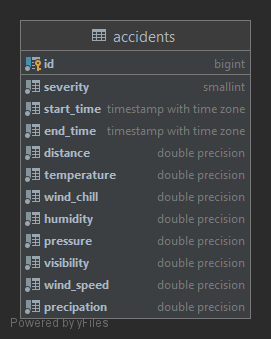
\includegraphics[width=14cm]{accidents.png}
 \vspace{-0.3cm}
 \caption{Tabela reprezentująca omawiane dane wykonana w DBMS Postgresql}
 \label{Wynik klasyfikacji.}
\end{figure}
\newpage


%%%%%%%%%%%%%%%%%%%%%%%%%%%%%%%%%%%%%%%%
\section{Atrybuty i liczności obiektów wyrażone zmiennymi lingwistycznymi}

Poniżej zostaną przedstawione zmiene lingwistyczne\cite{niewiadomskiRozmyte} dla jedenastu atrybutów z bazy danych wraz z przypisanymi etykietami w formie funkcji przynależności oraz wzorów analitycznych. \\

%%%%%%%%%%%%%%%%%%%%%%%%%%%%%%%%%%%%%%%
Na podstawie znajdujących się w bazie danych pól Czas rozpoczęcia (Start\_Time) oraz Czas zakończenia (End\_Time) zostanie obliczony Czas utrudnień w ruchu drogowym (Duration) spowodowanych przez wypadek według wzoru:
\begin{equation}
Duration = End\_Time - Start\_Time
\end{equation}
Przedstawienie Czasu utrudnień w ruchu drogowym (Duration) spowodowanych przez wypadek jako zmiennej lingwistycznej. Do zmiennej lingwistycznej zostały dopasowane etykiety: krótki, średni, długi. 
\begin{equation}
\mu _{czasTrwaniaPonizejGodziny}(x) =  \left\{ \begin{array}{rcl}
\frac{1 - x}{1} & \mbox{dla} & 0 < x \leq 1\\
\end{array}\right.
\end{equation}

\begin{equation}
\mu _{czasTrwaniaOkoloDwochGodzin}(x) =  \left\{ \begin{array}{rcl}
\frac{x}{2} & \mbox{dla} & 0 < x \leq 2\\
\frac{4 - x}{2} & \mbox{dla} & 2 < x \leq 4\\
\end{array}\right.
\end{equation}

\begin{equation}
\mu _{czasTrwaniaOkoloCzterechGodzin}(x) =  \left\{ \begin{array}{rcl}
\frac{x - 2}{2} & \mbox{dla} & 2 < x \leq 4\\
\frac{6 - x}{2} & \mbox{dla} & 4 < x \leq 6\\
\end{array}\right.
\end{equation}

\begin{equation}
\mu _{czasTrwaniaOkoloSzesciuGodzin}(x) =  \left\{ \begin{array}{rcl}
\frac{x - 4}{2} & \mbox{dla} & 4 < x \leq 6\\
\frac{8 - x}{2} & \mbox{dla} & 6 < x \leq 8\\
\end{array}\right.
\end{equation}

\begin{equation}
\mu _{czasTrwaniaPonadSzescGodzin}(x) =  \left\{ \begin{array}{rcl}
\frac{x - 6}{2} & \mbox{dla} & 6 < x \leq 8\\
 1 & \mbox{dla} & 8 \leq  x \\
\end{array}\right.
\end{equation}

gdzie: \(\mu _{czasTrwaniaPonizejGodziny}\), \(\mu _{czasTrwaniaOkoloDwochGodzin}\), \(\mu _{czasTrwaniaOkoloCzterechGodzin}\), \(\mu _{czasTrwaniaOkoloSzesciuGodzin}\), \(\mu _{czasTrwaniaPonadSzescGodzin}\) - funkcje przynależności, \textit{x} - czas trwania wypadku. 
\begin{figure}[h!]
 \centering
 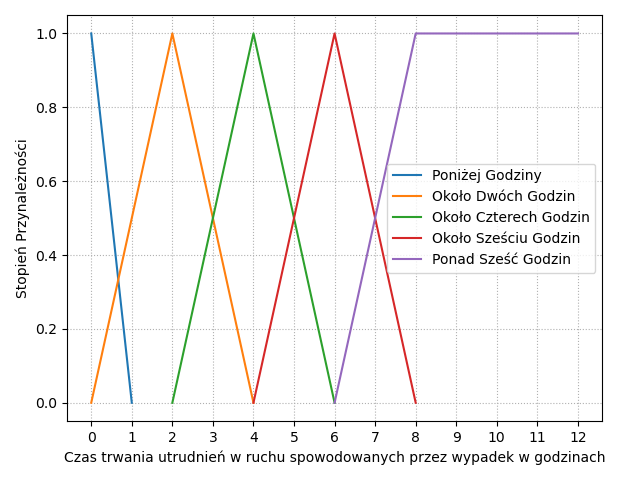
\includegraphics[width=14cm]{FunkcjaPrzynaleznosciCzasTrwania.png}
 \vspace{-0.3cm}
 \caption{Wykres funkcji przynależności zbiorów rozmytych ilustrujących wartości zmiennej lingwistycznej czas utrudnień w ruchu drogowym (Duration) spowodowanych przez wypadek. }
 \label{rysunek do eksperymentu 1 wariantu 1}
\end{figure}
\newpage


%%%%%%%%%%%%%%%%%%%%%%%%%%%%%%%%%%%%%%%%
Przedstawienie odległości jako zmiennej lingwistycznej. Do zmiennej lingwistycznej zostały dopasowane etykiety: krótki, długi. 
\begin{equation}
\mu _{OdlegloscPonizejPolMili}(x) =  \left\{ \begin{array}{rcl}
 1 & \mbox{dla} & x  \leq 0.5 \\
\end{array}\right.
\end{equation}

\begin{equation}
\mu _{OdlegloscOkoloJednejMili}(x) =  \left\{ \begin{array}{rcl}
x & \mbox{dla} & 0 < x \leq 1\\
2 - x & \mbox{dla} & 1 < x \leq 2\\
\end{array}\right.
\end{equation}

\begin{equation}
\mu _{OdlegloscOkoloTrzechMili}(x) =  \left\{ \begin{array}{rcl}
\frac{x - 1}{2} & \mbox{dla} & 1 < x \leq 3\\
\frac{5 - x}{2} & \mbox{dla} & 3 < x \leq 5\\
\end{array}\right.
\end{equation}

\begin{equation}
\mu _{OdlegloscPonadTrzyMile}(x) =  \left\{ \begin{array}{rcl}
\frac{x - 3}{2} & \mbox{dla} & 3 < x \leq 5\\
1 & \mbox{dla} & 5 \leq x \\
\end{array}\right.
\end{equation}

gdzie: \(\mu _{OdlegloscPonizejPolMili}\), \(\mu _{OdlegloscOkoloJednejMili}\), \(\mu _{OdlegloscOkoloTrzechMili}\), \(\mu _{OdlegloscPonadTrzyMile}\) - funkcje przynależności, \textit{x} - odleglość. 

\begin{figure}[h!]
 \centering
 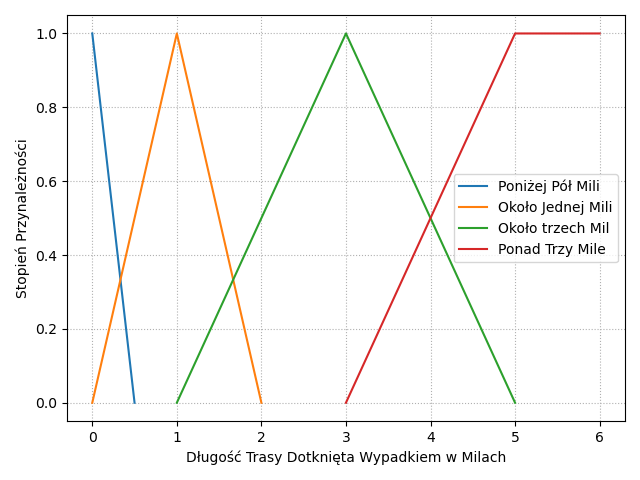
\includegraphics[width=14cm]{FunkcjaPrzynaleznosciOdleglosc.png}
 \vspace{-0.3cm}
 \caption{Wykres funkcji przynależności zbiorów rozmytych ilustrujących wartości zmiennej lingwistycznej odległości. }
 \label{rysunek do eksperymentu 1 wariantu 1}
\end{figure}
\newpage

%%%%%%%%%%%%%%%%%%%%%%%%%%%%%%%%%%%%%%%%
Przedstawienie temperatury oraz temperatury odczuwalnej jako zmiennej lingwistycznej. Do zmiennej lingwistycznej zostały dopasowane etykiety: bardzo zimno, zimno, umiarkowanie, ciepło, bardzo ciepło. 
\begin{equation}
\mu _{temperaturaBardzoZimno}(x) =  \left\{ \begin{array}{rcl}
 1 & \mbox{dla} & x  \leq 14 \\
\frac{23 - x}{9} & \mbox{dla} & 14 < x \leq 23\\
\end{array}\right.
\end{equation}

\begin{equation}
\mu _{temperaturaZimno}(x) =  \left\{ \begin{array}{rcl}
\frac{x - 14}{9} & \mbox{dla} & 14 < x \leq 23\\
1 & \mbox{dla} & 23 < x < 44\\
\frac{54 - x}{10} & \mbox{dla} & 44 < x \leq 54\\
\end{array}\right.
\end{equation}

\begin{equation}
\mu _{temperaturaUmiarkowanie}(x) =  \left\{ \begin{array}{rcl}
\frac{x - 44}{10} & \mbox{dla} & 44 < x \leq 54\\
1 & \mbox{dla} & 54 < x < 63\\
\frac{71 - x}{8} & \mbox{dla} & 63 < x \leq 71\\
\end{array}\right.
\end{equation}

\begin{equation}
\mu _{temperaturaCieplo}(x) =  \left\{ \begin{array}{rcl}
\frac{x - 63}{8} & \mbox{dla} & 63 < x \leq 71\\
1 & \mbox{dla} & 71 < x < 80\\
\frac{90 - x}{10} & \mbox{dla} & 80 < x \leq 90\\
\end{array}\right.
\end{equation}

\begin{equation}
\mu _{temperaturaBardzoCieplo}(x) =  \left\{ \begin{array}{rcl}
\frac{x - 80}{10} & \mbox{dla} & 80 < x \leq 90\\
1 & \mbox{dla} & 90 \leq x\\
\end{array}\right.
\end{equation}

gdzie: \(\mu _{temperaturaBardzoZimna}\), \(\mu _{temperaturaZimna}\), \(\mu _{temperaturaUmiarkowana}\), \(\mu _{temperaturaCiepla}\), \(\mu _{temperaturaBardzoCiepla}\) - funkcje przynależności, \textit{x} - temperatura, temperatura odczuwalna. 


\begin{figure}[h!]
 \centering
 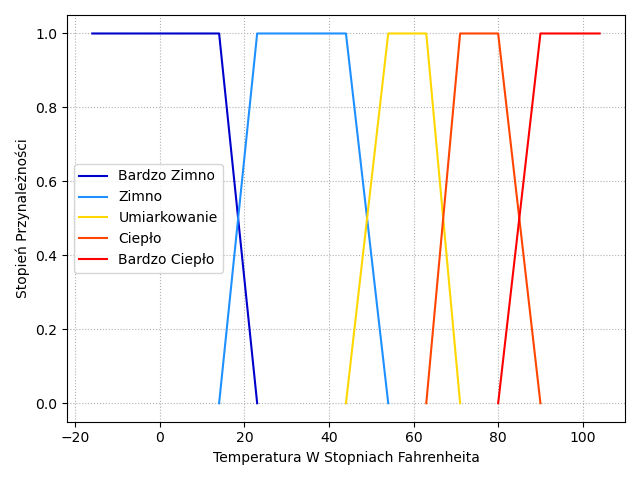
\includegraphics[width=14cm]{FunkcjaPrzynaleznosciTemperatura.png}
 \vspace{-0.3cm}
 \caption{Wykres funkcji przynależności zbiorów rozmytych ilustrujących wartości zmiennej lingwistycznej temperatury. }
 \label{rysunek do eksperymentu 1 wariantu 1}
\end{figure}
\newpage



%%%%%%%%%%%%%%%%%%%%%%%%%%%%%%%%%%%%%%%%
Przedstawienie wilgotności jako zmiennej lingwistycznej. Do zmiennej lingwistycznej zostały dopasowane etykiety: suche, umiarkowane, wilgotne. 

\begin{equation}
\mu _{wilgotnoscBardzoSuche}(x) =  \left\{ \begin{array}{rcl}
\frac{20 - x}{20} & \mbox{dla} & x \leq 20\\
\end{array}\right.
\end{equation}

\begin{equation}
\mu _{wilgotnoscSuche}(x) =  \left\{ \begin{array}{rcl}
\frac{x - 20}{20} & \mbox{dla} & 4 < x \leq 20\\
 1 & \mbox{dla} & 20 < x < 30 \\
\frac{30 - x}{10} & \mbox{dla} & 30 < x \leq 40\\
\end{array}\right.
\end{equation}

\begin{equation}
\mu _{wilgotnoscUmiarkowane}(x) =  \left\{ \begin{array}{rcl}
\frac{x - 30}{10} & \mbox{dla} & 30 < x \leq 40\\
1 & \mbox{dla} & 40 < x < 60\\
\frac{70 - x}{10} & \mbox{dla} & 60 < x \leq 70\\
\end{array}\right.
\end{equation}

\begin{equation}
\mu _{wilgotnoscWilgotne}(x) =  \left\{ \begin{array}{rcl}
\frac{x - 60}{10} & \mbox{dla} & 60 < x \leq 70\\
1 & \mbox{dla} & 70 \leq x\\
\end{array}\right.
\end{equation}

\begin{equation}
\mu _{wilgotnoscBardzoWilgotne}(x) =  \left\{ \begin{array}{rcl}
\frac{x - 60}{10} & \mbox{dla} & 60 < x \leq 70\\
1 & \mbox{dla} & 70 < x < 80\\
\frac{90 - x}{10} & \mbox{dla} & 80 < x \leq 90\\
\end{array}\right.
\end{equation}

gdzie: \(\mu _{wilgotnoscBardzoSuche}\), \(\mu _{wilgotnoscSuche}\), \(\mu _{wilgotnoscUmiarkowane}\), \(\mu _{wilgotnoscWilgotne}\), \(\mu _{wilgotnoscBardzoWilgotne}\) - funkcje przynależności, \textit{x} - wilgotność. 

\begin{figure}[h!]
 \centering
 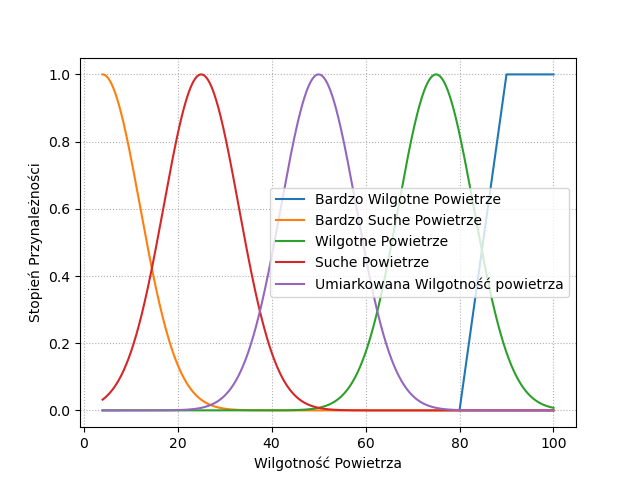
\includegraphics[width=14cm]{FunkcjaPrzynaleznosciWilgotnosc.png}
 \vspace{-0.3cm}
 \caption{Wykres funkcji przynależności zbiorów rozmytych ilustrujących wartości zmiennej lingwistycznej wilgotności. }
 \label{rysunek do eksperymentu 1 wariantu 1}
\end{figure}
\newpage


%%%%%%%%%%%%%%%%%%%%%%%%%%%%%%%%%%%%%%%%
Przedstawienie ciśnienia jako zmiennej lingwistycznej. Do zmiennej lingwistycznej zostały dopasowane etykiety: niskie, umiarkowane, wysokie. 
\begin{equation}
\mu _{cisnienieBardzoNiskie}(x) =  \left\{ \begin{array}{rcl}
 1 & \mbox{dla} & x  \leq 27 \\
\frac{27 - x}{0.5} & \mbox{dla} & 27 < x \leq 27.5\\
\end{array}\right.
\end{equation}

\begin{equation}
\mu _{cisnienieNiskie}(x) =  \left\{ \begin{array}{rcl}
\frac{x - 27.5}{0.5} & \mbox{dla} & 27 < x \leq 27.5\\
1 & \mbox{dla} & 27.5 < x < 28\\
\frac{28.5 - x}{0.5} & \mbox{dla} & 28 < x \leq 28.5\\
\end{array}\right.
\end{equation}

\begin{equation}
\mu _{cisnienieUmiarkowane}(x) =  \left\{ \begin{array}{rcl}
\frac{x - 28}{0.5} & \mbox{dla} & 28 < x \leq 28.5\\
1 & \mbox{dla} & 28.5 < x < 29\\
\frac{29.5 - x}{0.5} & \mbox{dla} & 29 < x \leq 29.5\\
\end{array}\right.
\end{equation}

\begin{equation}
\mu _{cisnienieWysokie}(x) =  \left\{ \begin{array}{rcl}
\frac{x - 30}{0.5} & \mbox{dla} & 29 < x \leq 29.5\\
1 & \mbox{dla} & 29.5 < x < 30\\
\frac{30.5 - x}{0.5} & \mbox{dla} & 30 < x \leq 30.5\\
\end{array}\right.
\end{equation}

\begin{equation}
\mu _{cisnienieBardzoWysokie}(x) =  \left\{ \begin{array}{rcl}
\frac{x - 30}{0.5} & \mbox{dla} & 30 < x \leq 30.5\\
1 & \mbox{dla} & 30.5 \leq x\\
\end{array}\right.
\end{equation}


gdzie: \(\mu _{cisnienieBardzoNiskie}\), \(\mu _{cisnienieNiskie}\), \(\mu _{cisnienieUmiarkowane}\), \(\mu _{cisnienieWysokie}\), \(\mu _{cisnienieBardzoWysokie}\) - funkcje przynależności, \textit{x} - ciśnienie. 

\begin{figure}[h!]
 \centering
 \includegraphics[width=14cm]{FunkcjaPrzynaleznosciCiśnienie.png}
 \vspace{-0.3cm}
 \caption{Wykres funkcji przynależności zbiorów rozmytych ilustrujących wartości zmiennej lingwistycznej ciśneinia. }
 \label{rysunek do eksperymentu 1 wariantu 1}
\end{figure}
\newpage



%%%%%%%%%%%%%%%%%%%%%%%%%%%%%%%%%%%%%%%%
Przedstawienie widoczności jako zmiennej lingwistycznej. Do zmiennej lingwistycznej zostały dopasowane etykiety: brak, słaba, ograniczona, dobra. 
\begin{equation}
\mu _{widocznoscBrak}(x) =   1 \ \ dla \ \ x  = 0
\end{equation}

\begin{equation}
\mu _{widocznoscSlaba}(x) =  \left\{ \begin{array}{rcl}
 1 & \mbox{dla} & x  \leq 0.1 \\
\frac{0.1 - x}{0.2} & \mbox{dla} & 0.1 < x \leq 0.3\\
\end{array}\right.
\end{equation}

\begin{equation}
\mu _{widocznoscOgraniczona}(x) =  \left\{ \begin{array}{rcl}
\frac{x - 0.1}{0.2} & \mbox{dla} & 0.1 < x \leq 0.3\\
1 & \mbox{dla} & 0.3 < x < 0.7\\
\frac{1 - x}{0.3} & \mbox{dla} & 0.7 < x \leq1\\
\end{array}\right.
\end{equation}

\begin{equation}
\mu _{widocznoscDobra}(x) =  \left\{ \begin{array}{rcl}
\frac{x - 0.7}{0.3} & \mbox{dla} & 0.7 < x \leq 1\\
1 & \mbox{dla} & 1 < x < 2\\
\frac{3 - x}{1} & \mbox{dla} & 2 < x \leq 3\\
\end{array}\right.
\end{equation}

\begin{equation}
\mu _{widocznoscPelna}(x) =  \left\{ \begin{array}{rcl}
\frac{x - 3}{1} & \mbox{dla} & 2 < x \leq 3\\
1 & \mbox{dla} & 3 \leq x\\
\end{array}\right.
\end{equation}

gdzie: \(\mu _{widocznoscBrak}\), \(\mu _{widocznoscSlaba}\), \(\mu _{widocznoscOgraniczona}\), \(\mu _{widocznoscDobra}\), \(\mu _{widocznoscPelna}\)  - funkcje przynależności, \textit{x} - widoczność. 

\begin{figure}[h!]
 \centering
 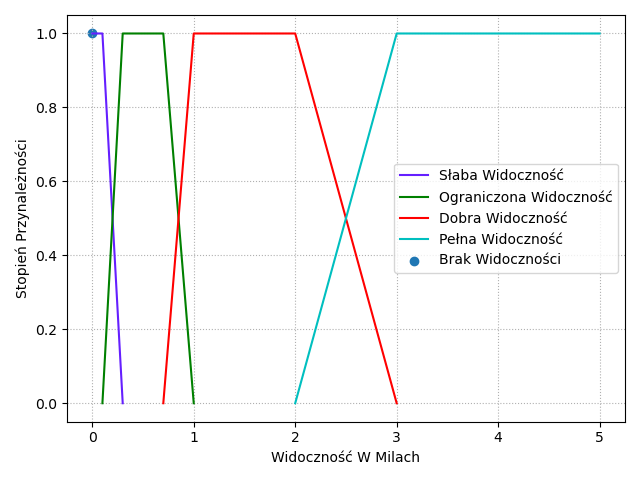
\includegraphics[width=14cm]{FunkcjaPrzynaleznosciWidocznosc.png}
 \vspace{-0.3cm}
 \caption{Wykres funkcji przynależności zbiorów rozmytych ilustrujących wartości zmiennej lingwistycznej widoczności. }
 \label{rysunek do eksperymentu 1 wariantu 1}
\end{figure}
\newpage


%%%%%%%%%%%%%%%%%%%%%%%%%%%%%%%%%%%%%%%%
Przedstawienie predkości wiatru jako zmiennej lingwistycznej. Do zmiennej lingwistycznej zostały dopasowane etykiety: brak, słaby, umiarkowany, silny, wicher, huragan. 

\begin{equation}
\mu _{wiatrBrak}(x) =   1 \ \ dla \ \ x  = 0
\end{equation}

\begin{equation}
\mu _{wiatrSlaby}(x) =  \left\{ \begin{array}{rcl}
 1 & \mbox{dla} & x  \leq 3 \\
\frac{3- x}{0.5} & \mbox{dla} & 3 < x \leq 3.5\\
\end{array}\right.
\end{equation}

\begin{equation}
\mu _{wiatrUmiarkowany}(x) =  \left\{ \begin{array}{rcl}
\frac{x - 3}{0.5} & \mbox{dla} & 3 < x \leq 3.5\\
1 & \mbox{dla} & 3.5 < x < 8\\
\frac{9 - x}{1} & \mbox{dla} & 8 < x \leq 9\\
\end{array}\right.
\end{equation}

\begin{equation}
\mu _{wiatrSilny}(x) =  \left\{ \begin{array}{rcl}
\frac{x - 8}{1} & \mbox{dla} & 8 < x \leq 9\\
1 & \mbox{dla} & 9 < x < 17\\
\frac{20 - x}{3} & \mbox{dla} & 17 < x \leq 20\\
\end{array}\right.
\end{equation}

\begin{equation}
\mu _{wiatrWicher}(x) =  \left\{ \begin{array}{rcl}
\frac{x - 17}{3} & \mbox{dla} & 17 < x \leq 20\\
1 & \mbox{dla} & 20 < x < 27\\
\frac{30 - x}{3} & \mbox{dla} & 27 < x \leq 30\\
\end{array}\right.
\end{equation}

\begin{equation}
\mu _{wiatrHuragan}(x) =  \left\{ \begin{array}{rcl}
\frac{x - 40}{10} & \mbox{dla} & 30 < x \leq 40\\
1 & \mbox{dla} & 40 \leq x\\
\end{array}\right.
\end{equation}

gdzie: \(\mu _{wiatrBrak}\), \(\mu _{wiatrSlaby}\), \(\mu _{wiatrUmiarkowany}\), \(\mu _{wiatrSilny}\), \(\mu _{wiatrWicher}\), \(\mu _{wiatrHuragan}\)  - funkcje przynależności, \textit{x} - prędkość wiatru. 

\begin{figure}[h!]
 \centering
 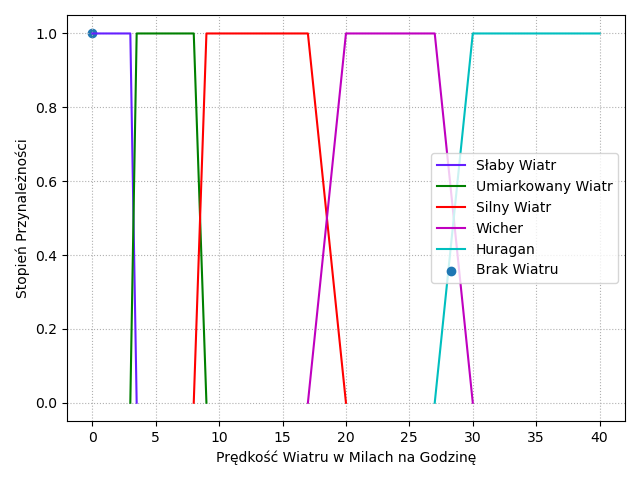
\includegraphics[width=14cm]{FunkcjaPrzynaleznosciPredkoscWiatru.png}
 \vspace{-0.3cm}
 \caption{Wykres funkcji przynależności zbiorów rozmytych ilustrujących wartości zmiennej lingwistycznej prędkości wiatru. }
 \label{rysunek do eksperymentu 1 wariantu 1}
\end{figure}
\newpage



%%%%%%%%%%%%%%%%%%%%%%%%%%%%%%%%%%%%%%%%
Przedstawienie opadów jako zmiennej lingwistycznej. Do zmiennej lingwistycznej zostały dopasowane etykiety: brak, niewielkie, umiarkowane, duże. 

\begin{equation}
\mu _{opadyBrak}(x) =   1 \ \ dla \ \ x  = 0
\end{equation}

\begin{equation}
\mu _{opadyNiewielkie}(x) =  \left\{ \begin{array}{rcl}
 1 & \mbox{dla} & x  \leq 0.1 \\
\frac{0.1- x}{0.1} & \mbox{dla} & 0.1 < x \leq 0.2\\
\end{array}\right.
\end{equation}

\begin{equation}
\mu _{opadyUmiarkowane}(x) =  \left\{ \begin{array}{rcl}
\frac{x - 0.1}{0.1} & \mbox{dla} & 0.1 < x \leq 0.2\\
1 & \mbox{dla} & 0.2 < x < 0.3\\
\frac{0.35 - x}{0.05} & \mbox{dla} & 0.3 < x \leq 0.35\\
\end{array}\right.
\end{equation}


\begin{equation}
\mu _{opadyDuze}(x) =  \left\{ \begin{array}{rcl}
\frac{x - 0.35}{0.05} & \mbox{dla} & 0.3 < x \leq 0.35\\
1 & \mbox{dla} & 0.35 < x < 0.4\\
\frac{0.45 - x}{0.05} & \mbox{dla} & 0.4 < x \leq 0.45\\
\end{array}\right.
\end{equation}

\begin{equation}
\mu _{opadyBardzoDuze}(x) =  \left\{ \begin{array}{rcl}
\frac{x - 0.4}{0.05} & \mbox{dla} & 0.4 < x \leq 0.45\\
1 & \mbox{dla} & 0.45 \leq x\\
\end{array}\right.
\end{equation}

gdzie: \(\mu _{opadyBrak}\), \(\mu _{opadyNiewielkie}\), \(\mu _{opadyUmiarkowane}\), \(\mu _{opadyDuze}\), \(\mu _{opadyBardzoDuze}\)  - funkcje przynależności, \textit{x} - opady. 

\begin{figure}[h!]
 \centering
 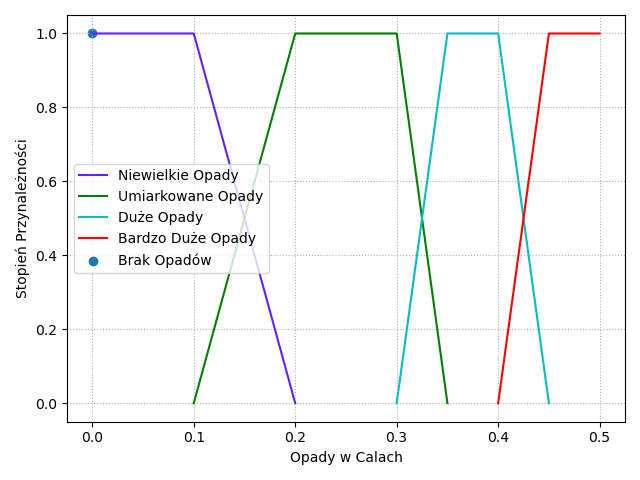
\includegraphics[width=14cm]{FunkcjaPrzynaleznosciOpady.png}
 \vspace{-0.3cm}
 \caption{Wykres funkcji przynależności zbiorów rozmytych ilustrujących wartości zmiennej lingwistycznej opadów. }
 \label{rysunek do eksperymentu 1 wariantu 1}
\end{figure}
\newpage


%%%%%%%%%%%%%%%%%%%%%%%%%%%%%%%%%%%%%%%%
Do kwantyfikatora lingwistycznego względnego\cite{niewiadomskiRozmyte} zostały dopasowane etykiety: niewiele, około 1/4, około połowy, większość, prawie wszystkie. 

\begin{equation}
\mu _{niewiele}(x) =   exp( \frac{- x^2}{0.02} )
\end{equation}

\begin{equation}
\mu _{okoloJednejCzwartej}(x) =   exp( \frac{- (x - 0.25)^2}{0.02} )
\end{equation}

\begin{equation}
\mu _{okoloPolowy}(x) =   exp( \frac{- (x - 0.5)^2}{0.02} )
\end{equation}

\begin{equation}
\mu _{wiekszosc}(x) =   exp( \frac{- (x - 0.75)^2}{0.02} )
\end{equation}

\begin{equation}
\mu _{prawieWszystkie}(x) =   exp( \frac{- (x - 1)^2}{0.02} )
\end{equation}

gdzie: \(\mu _{niewiele}\), \(\mu _{okoloJednejCzwartej}\), \(\mu _{okoloPolowy}\), \(\mu _{wiekszosc}\), \(\mu _{prawieWszystkie}\)  - kwantyfikatory, \textit{x} - stosunek liczby obiektów posiadających cechę do wszystkich rozważanych obiektów. 

\begin{figure}[h!]
 \centering
 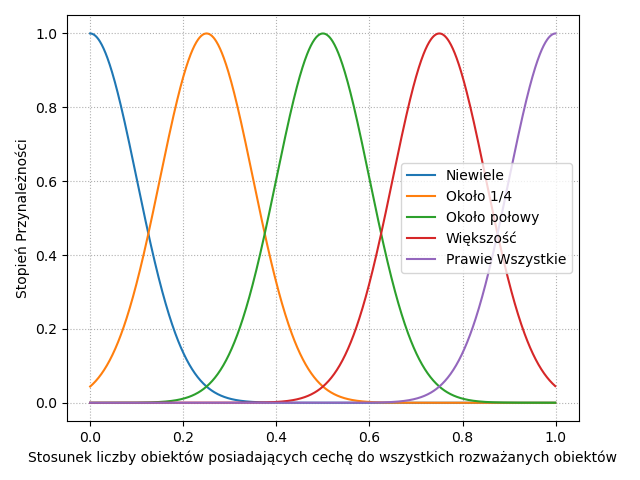
\includegraphics[width=14cm]{kwantyfikatory.png}
 \vspace{-0.3cm}
 \caption{Wykres funkcji przynależności kwantyfikatorów lingwistycznych względnych. }
 \label{rysunek do eksperymentu 1 wariantu 1}
\end{figure}
\newpage

%%%%%%%%%%%%%%%%%%%%%%%%%%%%%%%%%%%%%%%%
Do kwantyfikatora lingwistycznego absolutnego\cite{niewiadomskiRozmyte} zostały dopasowane etykiety: poniżej 10, około 50, około 100, między 100 a 200, około 200, ponad 200. 

\begin{equation}
\mu _{ponizej10}(x) =  \left\{ \begin{array}{rcl}
\frac{10 - x}{10} & \mbox{dla} & 0 < x \leq 10\\
\end{array}\right.
\end{equation}

\begin{equation}
\mu _{okolo10}(x) =  \left\{ \begin{array}{rcl}
\frac{x}{10} & \mbox{dla} & 0 < x \leq 10\\
\frac{20 - x}{10} & \mbox{dla} & 10 < x \leq 20\\
\end{array}\right.
\end{equation}

\begin{equation}
\mu _{okolo50}(x) =  \left\{ \begin{array}{rcl}
\frac{x - 10}{25} & \mbox{dla} & 10 < x \leq 35\\
1 & \mbox{dla} & 35 < x < 65\\
\frac{90 - x}{25} & \mbox{dla} & 65 < x \leq 90\\
\end{array}\right.
\end{equation}

\begin{equation}
\mu _{okolo100}(x) =  \left\{ \begin{array}{rcl}
\frac{x - 50}{40} & \mbox{dla} & 50 < x \leq 90\\
1 & \mbox{dla} & 90 < x < 110\\
\frac{150 - x}{50} & \mbox{dla} & 110 < x \leq 150\\
\end{array}\right.
\end{equation}

\begin{equation}
\mu _{miedzy100A200}(x) =  \left\{ \begin{array}{rcl}
\frac{x}{50} & \mbox{dla} & 100 < x \leq 150\\
\frac{200- x}{50} & \mbox{dla} & 150 < x \leq 200\\
\end{array}\right.
\end{equation}

\begin{equation}
\mu _{okolo200}(x) =  \left\{ \begin{array}{rcl}
\frac{x - 150}{40} & \mbox{dla} & 150 < x \leq 190\\
1 & \mbox{dla} & 190 < x < 210\\
\frac{250 - x}{40} & \mbox{dla} & 210 < x \leq 250\\
\end{array}\right.
\end{equation}

\begin{equation}
\mu _{Ponad200}(x) =  \left\{ \begin{array}{rcl}
\frac{x}{50} & \mbox{dla} & 200 < x \leq 250\\
1 & \mbox{dla} & 250 \leq x\\
\end{array}\right.
\end{equation}

gdzie: \(\mu _{ponizej10}\), \(\mu _{okolo10}\), \(\mu _{okolo50}\), \(\mu _{okolo100}\), \(\mu _{miedzy100A200}\), \(\mu _{okolo200}\), \(\mu _{Ponad200}\)  - kwantyfikatory absolutne, \textit{x} - absolutna wartość liczby obiektów posiadających cechę. 

\begin{figure}[h!]
 \centering
 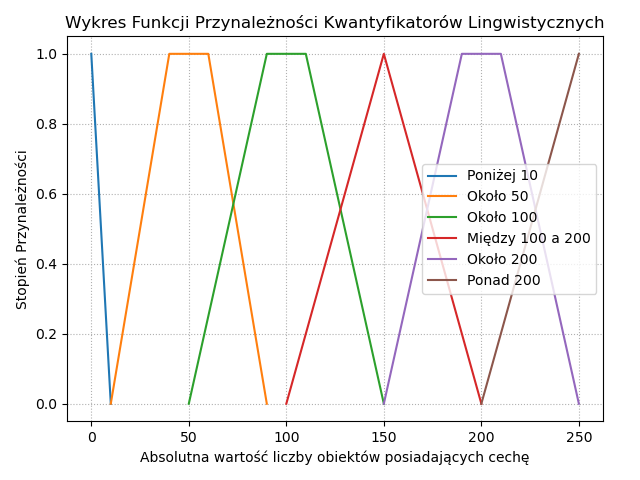
\includegraphics[width=14cm]{kwantyfikatory_absolutny.png}
 \vspace{-0.3cm}
 \caption{Wykres funkcji przynależności kwantyfikatorów lingwistycznych absolutnych. }
 \label{rysunek do eksperymentu 1 wariantu 1}
\end{figure}
\newpage

%%%%%%%%%%%%%%%%%%%%%%%%%%%%%%%%%%%%%%%%
\section{Narzędzia obliczeniowe: projekt (wybór, implementacja) i diagram UML pakietu obliczeń rozmytych. Diagram UML generatora podsumowań}
\subsection{Diagram pakietu obliczeń rozmytych}
W celu wykonania 


\newpage
Diagram UML i zwięzły opis pakietu obliczeń rozmytych: źródło pakietu
(zewnętrzny/własny/hybrydowy), przypis do literatury. Krótka charakterystyka
najważniejszych klas i podstawowych dla zadania ich metod. \\
\noindent {\bf Sekcja uzupełniona jako efekt zadania Tydzień 10 wg Harmonogramu Zajęć
na WIKAMP KSR.}

\subsection{Diagram UML generatora podsumowań. Krótka instrukcja użytkownika} 
Diagram UML generatora podsumowań (warstwy obliczeniowej oraz interfejsu
użytkownika). Krótki ilustrowany opis jak użytkownik może korzystać z aplikacji, w~szczególności
wprowadzać parametry  podsumowań, odczytywać wyniki oraz definiować własne etykiety i
kwantyfikatory. Wersja JRE i inne wymogi niezbędne do uruchomienia aplikacji przez użytkownika na własnym komputerze. \\
\noindent {\bf Sekcja uzupełniona jako efekt zadania Tydzień 11 wg Harmonogramu Zajęć
na WIKAMP KSR.}

\section{ Jednopodmiotowe podsumowania lingwistyczne. Miary jakości, podsumowanie optymalne}
Wyniki kolejnych eksperymentów wg punktów 2.-4. opisu projektu 2.  Listy podsumowań
jednopodmiotowych i tabele/rankingi podsumowań dla danych atrybutów obowiązkowe i dokładnie opisane w ,,captions'' (tytułach), konieczny opis kolumn i wierszy tabel. Dla każdego podsumowania podane miary jakości oraz miara jakości podsumowania
optymalnego.\\
\noindent {\bf Sekcja uzupełniona jako efekt zadania Tydzień 11 wg Harmonogramu Zajęć
na WIKAMP KSR.}



\section{Wielopodmiotowe podsumowania lingwistyczne i~ich miary jakości} 
Wyniki kolejnych eksperymentów wg punktów 2.-4. opisu projektu 2. Uzasadnienie i
metoda podziału zbioru danych na rozłączne podmioty. Listy podsumowań
wielopodmiotowych i tabele/rankingi podsumowań dla danych atrybutów obowiązkowe i
dokładnie opisane w ,,captions'' (tytułach), konieczny opis kolumn i wierszy tabel.
Konieczne uwzględnienie wszystkich 4-ch form podsumowań wielopodmiotowych. 
\\ 

** Możliwe sformułowanie zagadnienia wielopodmiotowego podsumowania optymalnego **.\\

{**Ewentualne wyniki realizacji punktu ,,na ocenę 5.0'' wg opisu Projektu 2. i ich porównanie do wyników z
części obowiązkowej**.}\\

\noindent {\bf Sekcja uzupełniona jako efekt zadania Tydzień 12 wg Harmonogramu Zajęć
na WIKAMP KSR.}


\section{Dyskusja, wnioski}
Dokładne interpretacje uzyskanych wyników w zależności od parametrów klasyfikacji
opisanych w punktach 3.-4 opisu Projektu 2. 
Szczególnie istotne są wnioski o charakterze uniwersalnym, istotne dla podobnych zadań. 
Omówić i wyjaśnić napotkane problemy (jeśli były). Każdy wniosek/problem powinien mieć poparcie
w przeprowadzonych eksperymentach (odwołania do konkretnych wyników: tabel i miar
jakości). Ocena które wybrane kwantyfikatory, sumaryzatory, kwalifikatory i/lub ich
miary jakości mają małe albo duże znaczenie dla wiarygodności i jakości otrzymanych
agregacji/podsumowań.  \\
\underline{Dla końcowej oceny jest to najważniejsza sekcja} sprawozdania, gdyż prezentuje poziom
zrozumienia rozwiązywanego problemu.\\

** Możliwości kontynuacji prac w obszarze logiki rozmytej i wnioskowania rozmytego, zwłaszcza w kontekście pracy inżynierskiej,
magisterskiej, naukowej, itp. **\\

\noindent {\bf Sekcja uzupełniona jako efekt zadań Tydzień 11 i Tydzień 12 wg
Harmonogramu Zajęć na WIKAMP KSR.}


\section{Braki w realizacji projektu 2.}
Wymienić wg opisu Projektu 2. wszystkie niezrealizowane obowiązkowe elementy projektu, ewentualnie
podać merytoryczne (ale nie czasowe) przyczyny tych braków. 


\begin{thebibliography}{99}
\bibitem{dane} 2021 Kaggle Inc [internetowa społeczność związana z analizą danych], US Accidents (3 million records -- updated)
A Countrywide Traffic Accident Dataset (2016 - 2020) [przeglądany 24 kwietnia 2021], Dostępny w: \url{https://www.kaggle.com/sobhanmoosavi/us-accidents}
Oficyna Wydawnicza EXIT, Warszawa, 2008.
\bibitem{fuzzy} Zadeh L.A., A computational approach to fuzzy quantifiers in natural languages. Computers and Maths with Applications, nr 9, 1983, 149-183
\bibitem{niewiadomskiRozmyte} A. Niewiadomski, Rozmyte metody inteligentnej interpretacji danych, tom 10, 2006, 546-547
 \bibitem{niewiadomski19} A. Niewiadomski, Zbiory rozmyte typu 2. Zastosowania w reprezentowaniu informacji.  Seria „Problemy współczesnej informatyki” pod redakcją L. Rutkowskiego. Akademicka Oficyna Wydawnicza EXIT, Warszawa, 2019.
\bibitem{zadrozny06} S. Zadrożny, Zapytania nieprecyzyjne i lingwistyczne podsumowania baz danych, EXIT, 2006, Warszawa
\bibitem{niewiadomski08} A. Niewiadomski, Methods for the Linguistic Summarization of Data: Applications of Fuzzy Sets and Their Extensions, Akademicka 
\end{thebibliography}

Literatura zawiera wyłącznie źródła recenzowane i/lub o potwierdzonej wiarygodności,
możliwe do weryfikacji i cytowane w sprawozdaniu. 
\end{document}
